\subsection{Partitions and Quotient Sets}

\begin{definition} \label{def:partition-of-a-set} \hlt{Partition of a Set}\\
Let $X$ be a set. A \hlt{partition} of $X$ is a set $\mathcal{F}\subseteq\mathcal{P}(X)\setminus\{\emptyset\}$ satisfying $(\forall x\in X)(\exists! B\in\mathcal{F})\,x\in B$.\\
The members of $\mathcal{F}$ are its \hlt{blocks}.
\end{definition}

\begin{proposition} \label{prop:equivalence-relations-partitions} \hlt{Equivalence Classes Partition the Set}\\
Let $X$ be a set, let $\sim$ be an equivalence relation on $X$, and set $\mathcal{F}_{\sim}\defeq\{[x]_{\sim}:x\in X\}$. Then $\mathcal{F}_{\sim}$ is a partition of $X$.
\begin{proof}
For $x\in X$, reflexivity gives $x\in[x]_{\sim}$; hence the classes are nonempty and cover $X$.\\
If $u\in[x]_{\sim}\cap[y]_{\sim}$, then $u\sim x$ and $u\sim y$, whence $x\sim y$ and $y\sim x$ by symmetry and transitivity.\\
If $v\in[x]_{\sim}$, then $v\sim x\sim y$, so $v\in[y]_{\sim}$. If $v\in[y]_{\sim}$, then $v\sim y\sim x$, so $v\in[x]_{\sim}$.\\
Thus intersecting classes are equal, proving unique class membership; hence $\mathcal{F}_{\sim}$ partitions $X$.\\
\hlt{Structural Commentary}: Reflexivity supplies classes; symmetry and transitivity collapse intersections.\\
\hlt{Key Insight}: Two classes sharing an element have the same members.\\
\end{proof}
\end{proposition}

\begin{illustrationfigure}[H]
  \centering
  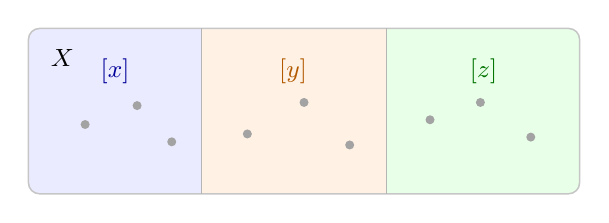
\begin{tikzpicture}[
  every node/.style={font=\small},
  ambient/.style={draw=gray!45, line width=0.55pt},
  seam/.style={draw=gray!58, line width=0.45pt},
  point/.style={circle, fill=gray!72, inner sep=1.15pt}
]
  \begin{scope}
    \clip[rounded corners=4pt] (0,0) rectangle (7.0,2.1);
    \fill[blue!8] (0,0) rectangle (2.2,2.1);
    \fill[orange!10] (2.2,0) rectangle (4.55,2.1);
    \fill[green!9] (4.55,0) rectangle (7.0,2.1);
  \end{scope}

  \draw[ambient, rounded corners=4pt] (0,0) rectangle (7.0,2.1);
  \draw[seam] (2.2,0) -- (2.2,2.1);
  \draw[seam] (4.55,0) -- (4.55,2.1);

  \node[anchor=north west] at (0.16,1.96) {$X$};
  \node[blue!60!black] at (1.10,1.55) {$[x]$};
  \node[orange!70!black] at (3.36,1.55) {$[y]$};
  \node[green!45!black] at (5.78,1.55) {$[z]$};

  \node[point] at (0.72,0.88) {};
  \node[point] at (1.38,1.12) {};
  \node[point] at (1.82,0.66) {};
  \node[point] at (2.78,0.76) {};
  \node[point] at (3.50,1.16) {};
  \node[point] at (4.08,0.62) {};
  \node[point] at (5.10,0.94) {};
  \node[point] at (5.74,1.16) {};
  \node[point] at (6.38,0.72) {};
\end{tikzpicture}

  \caption{Equivalence classes form disjoint blocks that cover the underlying set.}
  \label{fig:equivalence-classes-partition}
\end{illustrationfigure}

Figure \ref{fig:equivalence-classes-partition} depicts the partition in Proposition \ref{prop:equivalence-relations-partitions}. Every element of $X$ lies in one equivalence class, and distinct classes are disjoint.

\begin{proposition} \label{prop:partitions-determine-equivalence-relations} \hlt{Partitions Determine Equivalence Relations}\\
Let $X$ be a set and let $\mathcal{F}$ be a partition of $X$. For $x\in X$, let $B_x\in\mathcal{F}$ be the unique block containing $x$.\\
For $(x,y)\in X^2$, define $x\sim_{\mathcal{F}}y\Longleftrightarrow B_x=B_y$.
\begin{enumerate}[label=(\roman*)]
\setlength{\itemsep}{0pt}
\item \hlt{Equivalence relation}: $\sim_{\mathcal{F}}$ is an equivalence relation on $X$.
\item \hlt{Classes}: $(\forall x\in X)\,[x]_{\sim_{\mathcal{F}}}=B_x$, and $\{[x]_{\sim_{\mathcal{F}}}:x\in X\}=\mathcal{F}$.
\end{enumerate}
\begin{proof}
\begin{enumerate}[label=(\roman*)]
\setlength{\itemsep}{0pt}
\item For $x,y,z\in X$, $B_x=B_x$, so $x\sim_{\mathcal{F}}x$. If $x\sim_{\mathcal{F}}y$, then $B_x=B_y$, hence $B_y=B_x$ and $y\sim_{\mathcal{F}}x$.\\
Moreover, $(x\sim_{\mathcal{F}}y\land y\sim_{\mathcal{F}}z)\Rightarrow B_x=B_y=B_z\Rightarrow x\sim_{\mathcal{F}}z$. Thus $\sim_{\mathcal{F}}$ is reflexive, symmetric, and transitive.
\item Fix $x\in X$. If $y\in[x]_{\sim_{\mathcal{F}}}$, then $B_y=B_x$, so $y\in B_y=B_x$. If $y\in B_x$, then $B_x$ is a block containing $y$.\\
Uniqueness gives $B_y=B_x$, so $y\sim_{\mathcal{F}}x$ and $y\in[x]_{\sim_{\mathcal{F}}}$. Hence $[x]_{\sim_{\mathcal{F}}}=B_x$. Therefore $\{[x]_{\sim_{\mathcal{F}}}:x\in X\}\subseteq\mathcal{F}$.\\
If $B\in\mathcal{F}$, then $B\neq\emptyset$; choose $x\in B$. The uniqueness of $B_x$ gives $B=B_x=[x]_{\sim_{\mathcal{F}}}$, so the reverse containment holds.
\end{enumerate}
\hlt{Structural Commentary}: Block equality proves the axioms; uniqueness identifies classes with blocks.\\
\hlt{Key Insight}: Equivalent elements are assigned to the same block.
\end{proof}
\end{proposition}

\begin{example} \label{ex:rational-equivalence-classes-real-line} \hlt{Rational Equivalence on $\R$}\\
For $(x,y)\in\R^2$, define $x\sim_{\Q}y\Longleftrightarrow x-y\in\Q$. Fix $x,y,z\in\R$.
\begin{enumerate}[label=(\roman*)]
\setlength{\itemsep}{0pt}
\item \hlt{Reflexive}: $x-x=0\in\Q$.
\item \hlt{Symmetric}: $x-y\in\Q\Rightarrow y-x=-(x-y)\in\Q$.
\item \hlt{Transitive}: $(x-y\in\Q\land y-z\in\Q)\Rightarrow x-z=(x-y)+(y-z)\in\Q$.
\end{enumerate}
Thus $\sim_{\Q}$ is an equivalence relation, and $[x]_{\sim_{\Q}}=x+\Q=\{x+q:q\in\Q\}$.\\
A subset $\mathcal{R}\subseteq\R$ is a representative set iff $(\forall x\in\R)(\exists! r\in\mathcal{R})\,r\in x+\Q$.\\
\hlt{Key Insight}: Rational translation orbits are exactly the equivalence classes.
\end{example}

\begin{definition} \label{def:quotient-set-by-equivalence-relation} \hlt{Quotient Set}\\
Let $X$ be a set and let $\sim$ be an equivalence relation on $X$. The \hlt{quotient set} of $X$ by $\sim$ is $X/{\sim}\defeq\{[x]_{\sim}:x\in X\}$.
\end{definition}

\begin{proposition} \label{prop:quotient-map-well-defined-by-invariance} \hlt{Maps Defined on Equivalence Classes}\\
Let $X,Y$ be sets, let $\sim$ be an equivalence relation on $X$, and let $f:X\to Y$.\\
The assignment $g([x]_{\sim})\defeq f(x)$ defines $g:X/{\sim}\to Y$ iff $(\forall x,y\in X)\,[x\sim y\Rightarrow f(x)=f(y)]$.
\begin{proof}
\begin{enumerate}[label=(\roman*)]
\setlength{\itemsep}{0pt}
\item[$(\Rightarrow)$] Suppose $g$ is well-defined, $x\sim y$. Then $x\in[x]_{\sim}\cap[y]_{\sim}$, so $[x]_{\sim}=[y]_{\sim}$ by Proposition \ref{prop:equivalence-relations-partitions}. Thus $f(x)=g([x]_{\sim})=g([y]_{\sim})=f(y)$.
\item[$(\Leftarrow)$] Suppose $(\forall x,y\in X)\,[x\sim y\Rightarrow f(x)=f(y)]$. If $[x]_{\sim}=[y]_{\sim}$, then $x\in[y]_{\sim}$, whence $x\sim y$ and $f(x)=f(y)$.\\
Thus the assignment is independent of the representative. Hence it defines a map $g:X/{\sim}\to Y$.
\end{enumerate}
\hlt{Structural Commentary}: Equal classes prove necessity; representative independence proves sufficiency.\\
\hlt{Key Insight}: A class function cannot distinguish equivalent representatives.
\end{proof}
\end{proposition}
